\chapter{Concept Design}
\label{chp:ConceptDesign}
This chapter builds upon the knowledge gained in the literature review and explains the logic used to select the methods and sensors to realize each medical sign monitoring requirement of the Ear-Monitor. Selections will be made by analysing advantages and disadvantages of each option and combining it with sound engineering judgement.

\section{Temperature}
The Ear-Monitor will measure core temperature from the inside of the ear canal. The main criteria are sensor size and measurement accuracy. The method- and sensor selection are discussed separately.

\subsection{Temperature measurement method}
Two temperature measuring methods are considered, namely contact- and non-contact thermometers.

\subsubsection{Contact thermometers}
A contact RTD, thermocouple or thermistor is placed in contact with the canal wall, canal air or tympanic membrane. Table \ref{tab:ContactThermometers_Eval} summarises the evaluation.

\begin{table}[H]
\caption{Contact thermometers evaluation}
\label{tab:ContactThermometers_Eval}
\renewcommand{\arraystretch}{1.3}	%Wat doen hierdie?
\centering
\begin{tabular}{|Q{5cm}|Q{8cm}|} 
 \hline
\multicolumn{1}{|P{5cm}|}{\multirow{4}{*}{
\includegraphics[scale=1]{figs/Image.png}}}	& 	Advantages\\ 
							&	\tabitem Available in small sizes, ideal for the size restrictions of the ear canal.\\
  							&	\tabitem Good accuracy.\\
  							&	\tabitem Converting transducer voltage to temperature is simpler than with non-contact thermometers.\\
\hline
Sensor size: 0.5$\times$2.3 mm				& 	Disadvantages\\ 
Measurement accuracy: 0.15 $^{\circ}C$ 		&	\tabitem Canal wall and canal air temperature measurements can easily be influenced by ambient temperature conditions.\\
  											&	\tabitem Tympanic membrane contact can cause discomfort and harm to the wearer.\\
  											&	\tabitem More time is needed to take measurements, for the sensor needs to be in thermal equilibrium with the object.\\
 \hline
\end{tabular}
\end{table}

\subsubsection{Non-contact Thermometers}
A non-contact, infrared (IR) sensor is placed inside the ear canal and pointed at the tympanic membrane. Table \ref{tab:NonContactThermometers_Eval} summarises the evaluation.

\begin{table}[H]
\caption{Non-contact thermometers evaluation}
\label{tab:NonContactThermometers_Eval}
\renewcommand{\arraystretch}{1.3}	%Wat doen hierdie?
\centering
\begin{tabular}{|Q{5cm}|Q{8cm}|} 
 \hline
\multicolumn{1}{|P{5cm}|}{\multirow{4}{*}{
\includegraphics[scale=1]{figs/Image.png}}} 	& 	Advantages  \\ 
		&	\tabitem The sensor can measure the temperature of the tympanic membrane directly, which is the best representation of core temperature in the ear.\\
  		&	\tabitem Temperature conversion compensates for different ambient temperature conditions.\\
  		&	\tabitem No contact with the tympanic membrane lowers the injury risk to the user significantly.\\
\hline
Sensor size: 1.6 - 4 mm ${\diameter}$			&	Disadvantages  \\ 
Measurement accuracy: 0.2 - 0.5  $^{\circ}C$ 	&	\tabitem Non-contact temperature sensors are typically bigger than contact thermometers, adding to the size limitation challenge.\\
  												&	\tabitem If the tympanic membrane does not fill a considerable fraction of the sensor's field of view, erroneous measurements can occur.\\
 
 \hline
\end{tabular}
\end{table}

\subsubsection{Temperature measurement method choice}
A non-contact, IR sensor is selected for the Ear-Monitor. User safety, without significant performance compromise gives it superiority over contact thermometers for this application. The lower accuracy is justified by the fact that the tympanic membrane is a better representation of the core body temperature.

\subsection{Temperature measurement sensor}
To realize non-contact temperature measurement, two IR sensors are considered: The TMP006 from Texas Instruments and the ST60 Micro from Dexter Research Center Inc.

\subsubsection{ST60 Micro}
The ST60 Micro is a one channel, 80-junction, completely analogue temperature sensing device. It is enclosed in a Micro-TO package which is 4.09 mm in diameter as shown in Figure \ref{fig:ST60Micro}. The manufacturer emphasizes the ST60 Micro's versatility and proposes use in tympanic ear thermometers. A die temperature thermistor is available for ambient temperature compensation. Four wire are used to supply the sensor with power and to read transduced voltages.

 \begin{figure}[h]
   \centering
   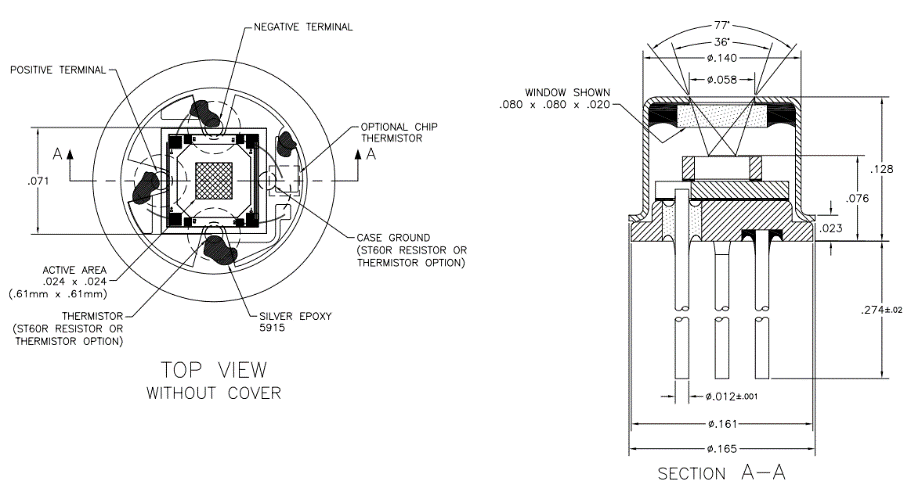
\includegraphics[scale=1]{figs/ST60Micro.png}
   \caption{ST60Micro diagram from the datasheet}
   \label{fig:ST60Micro}
\end{figure}

\subsubsection{TMP006}
The TMP006 is a fully integrated IR sensor measuring only 1.6$\times$1.6$\times$0.8 mm, ideally suited for a narrow ear canal. Thermophile voltage and sensor temperature, are made digitally available through hardware registers. These two values can be used to calculate the object temperature. Registers are accessed by a MCU though I\textsuperscript{2}C communication. Values are digitalized by a 16-bit on-chip ADC, eliminating the need for supporting analogue filters and amplifiers.
The TMP006's user guide suggest that is be used to calculate the surface temperature of target objects with emissivity values greater than 0.7, and preferably greater than 0.9. The literature study revealed that the emissivity of the eardrum is 0.98, placing it well within the required range.

\subsubsection{Temperature measurement sensor choice}
The simple shape of the ST60 Micro makes it easy to mount, but the diameter of the package may not fit in smaller ear canals and leave little room for the other sensors. Therefore, the ST60 Micro is eliminated.

\medskip

The smaller package size and on-chip ADC justifies the selection of the TMP006 for use in the Ear-Monitor. The TMP006 needs no separate analogue filter and amplifier. Furthermore, the manufacturer supplies detailed calibration documentation, allowing for more accurate and time effective calibration.

\section{Heart Rate}
The Ear-Monitor will extract heart rate from in or around the ear canal. The main criteria are sensor size, unobtrusiveness and the signal's susceptibility to noise. The method- and sensor selection are discussed separately. 

\subsection{Heart rate measurement method}

The following five methods from literature are considered to measure heart rate.

\subsubsection{Ear ECG}

As shown by \cite{winokur2012wearable}, an electrocardiogram can be detected behind the ear. One electrode is placed behind the ear on the mastoid bone and the other on the back of the neck. A differential amplifier and ADC is used to acquire the signal. Table \ref{tab:EarECG_Eval} summarises the evaluation.

\begin{table}[H]
\caption{Ear ECG}
\label{tab:EarECG_Eval}
\renewcommand{\arraystretch}{1.3}	%Wat doen hierdie?
\centering
\begin{tabular}{|Q{5cm}|Q{8cm}|} 
 \hline
\multicolumn{1}{|P{5cm}|}{\multirow{4}{*}{
\includegraphics[scale=1]{figs/Image.png}}} 						& 	Advantages  \\ 
  							&	\tabitem ECG is the standard method used by cardiologists to measure heart rate.\\
  							&	\tabitem Other cardiac information can be extracted from ECG i.e. heart rhythm, heart damage and the state of the conductive heart tissue.\\
  							&	\tabitem Not pulse transit time delay.\\
\hline
Sensor size: 10 mm  ${\diameter}$ electrodes					&	Disadvantages  \\ 
Unobtrusiveness: Bad - electrode needed behind ear and on neck 	&	\tabitem The sensor cannot be fitted entirely inside the ear canal.\\
Signal robustness: Noisy (Figure Winokur). 						&	\tabitem Two electrodes will be needed.\\
  																&	\tabitem Separate signal acquisition electronics are needed.\\
 
 \hline
\end{tabular}
\end{table}

\subsubsection{Ear PPG}
A LED and photodiode are used to detect variation in subcutaneous tissue blood volume due to the beating heart. Literature identifies three possible locations: Inside the ear canal, the earlobe and the concha. With unobtrusiveness in mind, the ear canal method is selected. This means reflective PPG is used. Table \ref{tab:EarPPG_Eval} summarises the evaluation.

\begin{table}[H]
\caption{Ear PPG}
\label{tab:EarPPG_Eval}
\renewcommand{\arraystretch}{1.3}	%Wat doen hierdie?
\centering
\begin{tabular}{|Q{5cm}|Q{8cm}|} 
 \hline
\multicolumn{1}{|P{5cm}|}{\multirow{4}{*}{
\includegraphics[scale=1]{figs/Image.png}}} 		& 	Advantages  \\ 
  			&	\tabitem A substantial pressure pulse can be detected in and around the ear.\\
  			&	\tabitem Pulse oximetry, a type of PPG, is a tried and tested way of measuring heart rate and SpO\textsubscript{2}.\\
  			&	\tabitem Respiratory related characteristics like amplitude modulation, respiratory-induced intensity variation and frequency modulation can be found only in PPG signals and can be used to determine respiratory rate.\\
\hline
Sensor size: Smallest - 1.9$\times$2.6$\times$0.8 mm		&	Disadvantages  \\ 
Unobtrusiveness: Good - fits inside ear canal 				&	\tabitem PPG is susceptible to motion artefacts and variation in blood profusion.\\
Signal noise: Low - clear pressure wave visible (Figure da2010ear) 						&	\tabitem Few PPG sensor packages are available to fit inside the ear canal.\\
  															&	\tabitem Using separate LEDs and photo detectors increases the complexity  and size for the proof of concept Ear-Monitor.\\
 
 \hline
\end{tabular}
\end{table}

\subsubsection{Ear BCG}
A pressure sensitive sensor or accelerometer is placed inside the ear canal to detect the mechanical effects of the pulsating heart. Table \ref{tab:EarBCG_Eval} summarises the evaluation.

\begin{table}[H]
\caption{Ear BCG}
\label{tab:EarBCG_Eval}
\renewcommand{\arraystretch}{1.3}	%Wat doen hierdie?
\centering
\begin{tabular}{|Q{5cm}|Q{8cm}|} 
 \hline
\multicolumn{1}{|P{5cm}|}{\multirow{3}{*}{
\includegraphics[scale=1]{figs/Image.png}}}		& 	Advantages  \\ 
  			&	\tabitem Pressure sensors can be made small enough for the limited space in the ear canal.\\
  			&	\tabitem Accelerometer can also be used to measure respiratory rate.\\
\hline
Sensor size: Smallest - 3$\times$3$\times$1 mm	[3]									&	Disadvantages  \\ 
Unobtrusiveness: A part of the sensor protrudes from the ear, can be made smaller 	&	\tabitem The signal detected by \cite{da2010ear} and \cite{winokur2012wearable} appears noisy and detecting beats will be troublesome.\\
Signal noise: High (da2010ear) (winokur2012wearable) 							&	\tabitem This method will be influenced by motion artefacts to such an extent that it will be unusable for most forms of practical use.\\
 
 \hline
\end{tabular}
\end{table}

\subsubsection{Phonocardiogram}
A microphone is placed inside the ear canal and identifies heart beats by analysing the sound produced by the cardiac cycle. Table \ref{tab:EarPhonocardiogram_Eval} summarises the evaluation.

\begin{table}[H]
\caption{Ear Phonocardiogram}
\label{tab:EarPhonocardiogram_Eval}
\renewcommand{\arraystretch}{1.3}	%Wat doen hierdie?
\centering
\begin{tabular}{|Q{5cm}|Q{8cm}|} 
 \hline
\multicolumn{1}{|P{5cm}|}{\multirow{2}{*}{
\includegraphics[scale=0.8]{figs/Image.png}}} 		& 	Advantages  \\ 
  			&	\tabitem Can be used to detect breathing as well, as shown by \cite{goverdovsky2016hearables}.\\
\hline
Sensor size: Smallest - 3.35$\times$2.5$\times$0.98 mm	&	Disadvantages  \\ 
Unobtrusiveness: Can fit inside the canal [5]			&	\tabitem Sounds from other sources like movement and speaking can corrupt the signal.\\
Signal noise: High 								&	\\
 
 \hline
\end{tabular}
\end{table}

\subsubsection{Heart rate method choice}
Ear PPG is selected as the Ear-Monitor's method of measuring heart rate. PPG produces a clear signal that will allow for accurate beat detection. This method can also be in cooperated into the $SpO_2$ measurement sensor, eliminating the need for two different sensors. The entire sensor can fit inside the ear canal making it unobtrusive. This method is also less susceptible to noise than ear BCG or a phonocardiogram.

\subsection{Heart rate measurement sensor}
Reflexive ear canal PPG is selected to measure heart rate. Three PPG sensors options are considered namely: separate LEDs and photodetector, the NJL5501R from JRC and the MAX30100 by Maxum Integrated.

\subsubsection{Separate LEDs and photodetector}
SMD LEDs is used along with one or more photo detectors. The components are mounted on a thin PCB and placed in the ear probe. The LEDs and photo detectors can be placed in various precise configurations and a wider choice of individual transducers can be used. Additional analogue electronics are needed to drive the LEDs, conditioning the detector signal output and compensate for ambient lighting. A commercial integrated analogue front end chip like Texas Instruments' AFE4400 can be used to perform this task.

\subsubsection{NJL5501R}
The NJL5501R is a surface mounted photo-emitter and -detector contained in one 1.9$\times$2.6$\times$0.8 mm package shown in Figure \ref{fig:NJL5501R}. Red and IR LEDs make it suitable for reflective pulse oximetry and heart beat detection. Its small size will allow it to fit in the ear canal while leaving adequate space for other sensors. It requires all the same supporting electronics as using the separate LEDs and a photo-detector method.

 \begin{figure}[h]
   \centering
   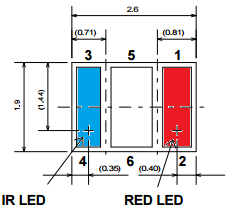
\includegraphics[scale=1]{figs/NJL5501R.png}
   \caption{NJL5501R diagram from the datasheet}
   \label{fig:NJL5501R}
\end{figure}

\subsubsection{MAX30100} 
The MAX30100 is single chip pulse oximeter and heart rate detector. It has red and IR LEDs, a photodetector, a 16-bit ADC and digital filters all in one 5.6$\times$2.8$\times$1.2 mm, 14-Pin package. The LEDs and photodetector are in the same plane, meaning it operates in reflective mode. Like the TMP006 is uses the I2C protocol to communicate with a MCU. Configuration registers allow the designer to specify sample rate, LED currents and LED pulse width. Figure \ref{fig:MAX30100_Diagram} shows a block diagram of the internal systems of the MAX30100.

\begin{figure}[H]
   \centering
   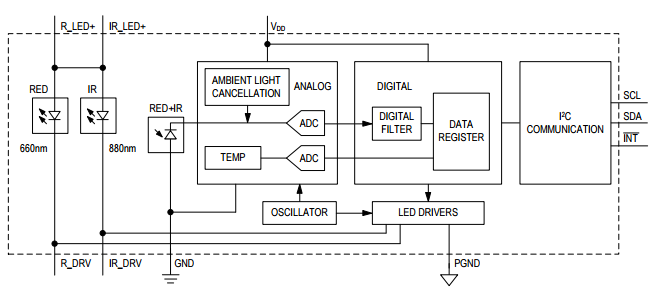
\includegraphics[scale=1]{figs/MAX30100_Diagram.png}
   \caption{MAX30100 block diagram from the datasheet}
   \label{fig:MAX30100_Diagram}
\end{figure}

The MAX30100 uses a 3.3V supply and programmable current sources to drive the LEDs, whilst digital operations are done at 1.8V. It draws between 6 and 12 mA while recording red and IR PPGs. It has a digital 50Hz/60Hz notch filter to reject powerline interference. LEDs can be individually supplied with 0 mA to 50 mA and LED pulse width can be varied from 0.2 ms to 1.6 ms. A sample rate can be chosen between 5 and 1000 samples per second. An important feature of the MAX30100 is its 64-byte deep FIFO register which is used to store the output values. Each output set consists of a 16-bit red and 16-bit IR value, meaning that there are 4 bytes per output and therefore 16 sets of output values can be held in the FIFO art any time. The MCU will read 4 bytes at a time from the FIFO to obtain the latest red and IR values.

\subsubsection{Heart rate sensor choice}
The MAX30100 is selected for use in the Ear-Monitor. It has optimized optics to guide outgoing and incoming light. It has integrated ambient light cancellation. Its entire AFE is integrated meaning that no additional electronics are needed, apart from the I2C lines and power regulators. This gives if a big advantage over the more complex separate LEDs and photodetector method. Its small size and reflective mode of operation, allows it to be placed inside of the ear canal. Data recorded by the MAX30100 will be used to calculate heart rate and SpO\textsubscript{2}. 

\section{Respiratory Rate}
The Ear-Monitor will measure respiratory rate from inside the ear canal. The main criteria are sensor size and susceptibility to noise corruption.

\subsection{Respiratory rate measuring method}
The following three respiratory rate measuring methods from literature are considered.

\subsubsection{Accelerometer}
A small MEMS accelerometer is placed inside the ear canal and measures the movement of the head due to breathing. Table \ref{tab:EarAccelerometer_Eval} summarises the evaluation.

\begin{table}[H]
\caption{Ear Accelerometer}
\label{tab:EarAccelerometer_Eval}
\renewcommand{\arraystretch}{1.3}	%Wat doen hierdie?
\centering
\begin{tabular}{|Q{5cm}|Q{8cm}|} 
 \hline
 Image 		& 	Advantages  \\ 
  			&	\tabitem The accelerometer can serve the dual purpose of measuring breathing and heart rate, thus saving space.\\
\hline
Sensor size: 3$\times$3$\times$1 mm	[3]					&	Disadvantages  \\ 
Noise: Very high							&	\tabitem This method is extremely vulnerable to noise form other movements.\\
 \hline
\end{tabular}
\end{table}

\subsubsection{Microphone}
A microphone is placed inside the ear canal and record the sound of air moving through the respiratory tracts, allowing the respiratory rate to be determined. Table \ref{tab:EarMicrophone_Eval} summarises the evaluation.

\begin{table}[H]
\caption{Ear Microphone}
\label{tab:EarMicrophone_Eval}
\renewcommand{\arraystretch}{1.3}	%Wat doen hierdie?
\centering
\begin{tabular}{|p{5cm}|p{8cm}|} 
 \hline
 Image 		& 	Advantages  \\ 
  			&	\tabitem The microphone can serve the dual purpose of measuring breathing and heart rate, thus saving space.\\
\hline
Sensor size: ?					&	Disadvantages  \\ 
Noise: Very high	&	\tabitem This method is extremely vulnerable to noise form other sounds like talking or ambient noise.\\
 \hline
\end{tabular}
\end{table}

\subsubsection{Respiratory related heart rate characteristics}
The variations in heart rate is used to determine the respiratory rate. These include amplitude modulation, respiratory-induced intensity variation and frequency modulation of the heart rate in synchronization with the respiration rate. Table \ref{tab:EarRRHRC_Eval} summarises the evaluation.

\begin{table}[H]
\caption{Respiratory related heart rate characteristics}
\label{tab:EarRRHRC_Eval}
\renewcommand{\arraystretch}{1.3}	%Wat doen hierdie?
\centering
\begin{tabular}{|Q{5cm}|Q{8cm}|} 
 \hline
 Image 		& 	Advantages  \\ 
  			&	\tabitem No dedicated sensor is needed.\\
  			&	\tabitem Less susceptible to noise the accelerometer or microphone method.\\
\hline
Sensor size: No sensor needed		&	Disadvantages  \\ 
Noise susceptibility: Low			&	\tabitem Only steady and relatively slow respiratory rates can be detected.\\
 \hline
\end{tabular}
\end{table}

\subsubsection{Respiratory rate choice}
The Ear-Monitor will determine respiratory rate by analysing respiratory related heart rate characteristics, of which heart rate frequency modulation through respiratory sinus arrhythmia (RSA) is found to be the most detectable. This method saves space by not requiring a dedicated sensor. It is also the lest susceptible to noise from other sources. No sensor selection is needed for this medical sign, as all the work is done by the micro controller.

\section{Blood oxygen saturation}
Pulse oximetry is the only practical way for the Ear-Monitor to measure blood oxygen saturation. The MAX30100 selected for measuring heart rate is equipped for this task. A red and IR LED as well as a photo-detector is available for the joint function for measuring heart rate and SpO\textsubscript{2}.

\section{Final concept}
The final concept is obtained by combining the methods and sensors selected in this chapter. To summarise: the Ear-Monitor will used the TMP006 IR sensor pointed at the tympanic membrane to measure core body temperature. The MAX30100 reflective pulse oximeter will be placed on on the side of the ear probe facing the canal wall. Red and IR PPGs from the MAX30100 will be used to extract heart rate and SpO\textsubscript{2}. Finally, respiratory rate will be determined by analysing the respiratory sinus arrhythmia.

\medskip

Additionally, a multi controller unit (MCU), battery and wireless transceiver are selected for the Ear-Monitor. The Arduino Pro Mini MCU has the necessary I/O pins for serial communication with the sensors and wireless module. It is also easy to program, making it ideal for the proof of concept version of the Ear-Monitor. Lithium polymer (LiPo) batteries are currently the best choice while regarding capacity, compactness, rechargeability and price and is therefore selected to supply the power to the Ear-Monitor. Bluetooth is the typically used standard for transmitting data over short distances and is supported by most modern smart devices. The HC-05 Bluetooth modem is selected and will allow the Ear-Monitor to send data to a supporting device through a wireless connection. Figure \ref{fig:EarMonitor_Concept} shows a diagram of the Ear-Monitor concept with a more detailed drawing of the ear probe with the selected sensors.


\begin{figure}[H]
   \centering
   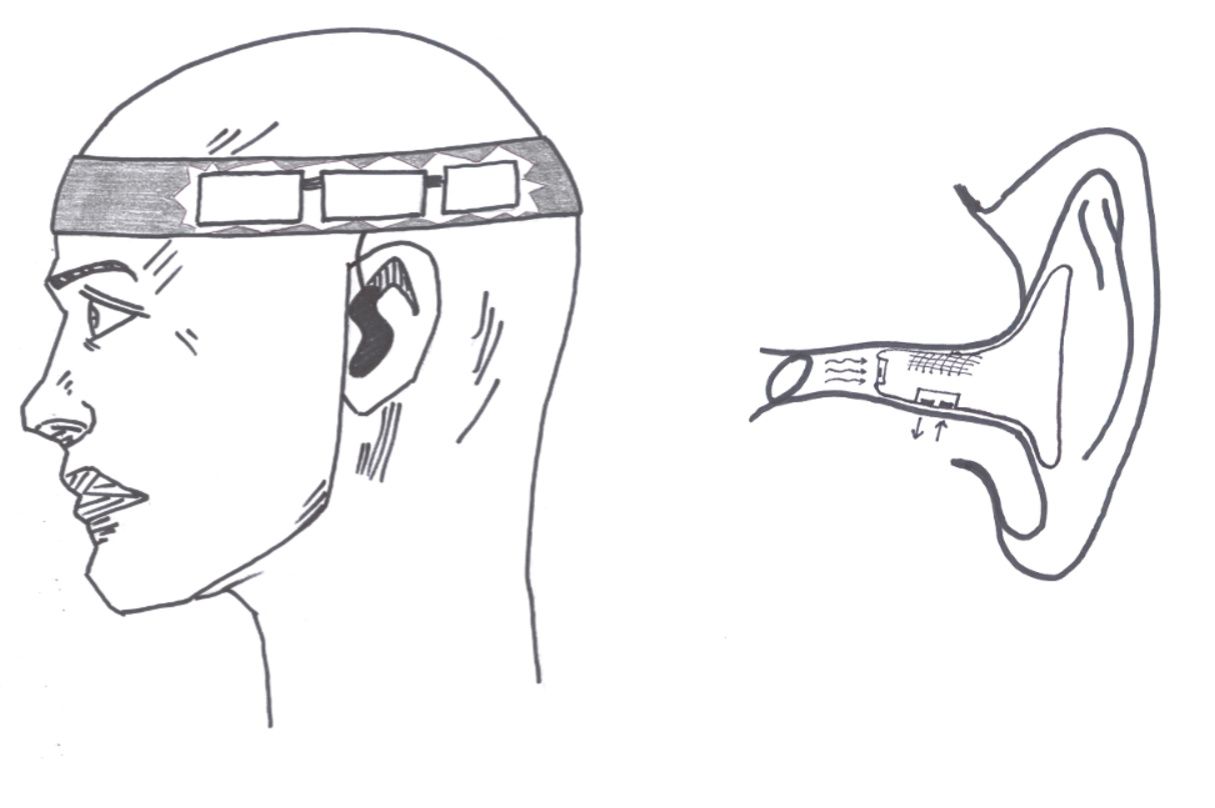
\includegraphics[scale=0.6]{figs/EarMonitor_Concept.pdf}
   \caption{(Add caption and labels on image)}
   \label{fig:EarMonitor_Concept}
\end{figure}
